\chapter{Area exploration}\label{chap:area_exploration}
different time exploration
imu to switch off
time following

\section{State machine}


\begin{figure}[!ht]
    \centering
    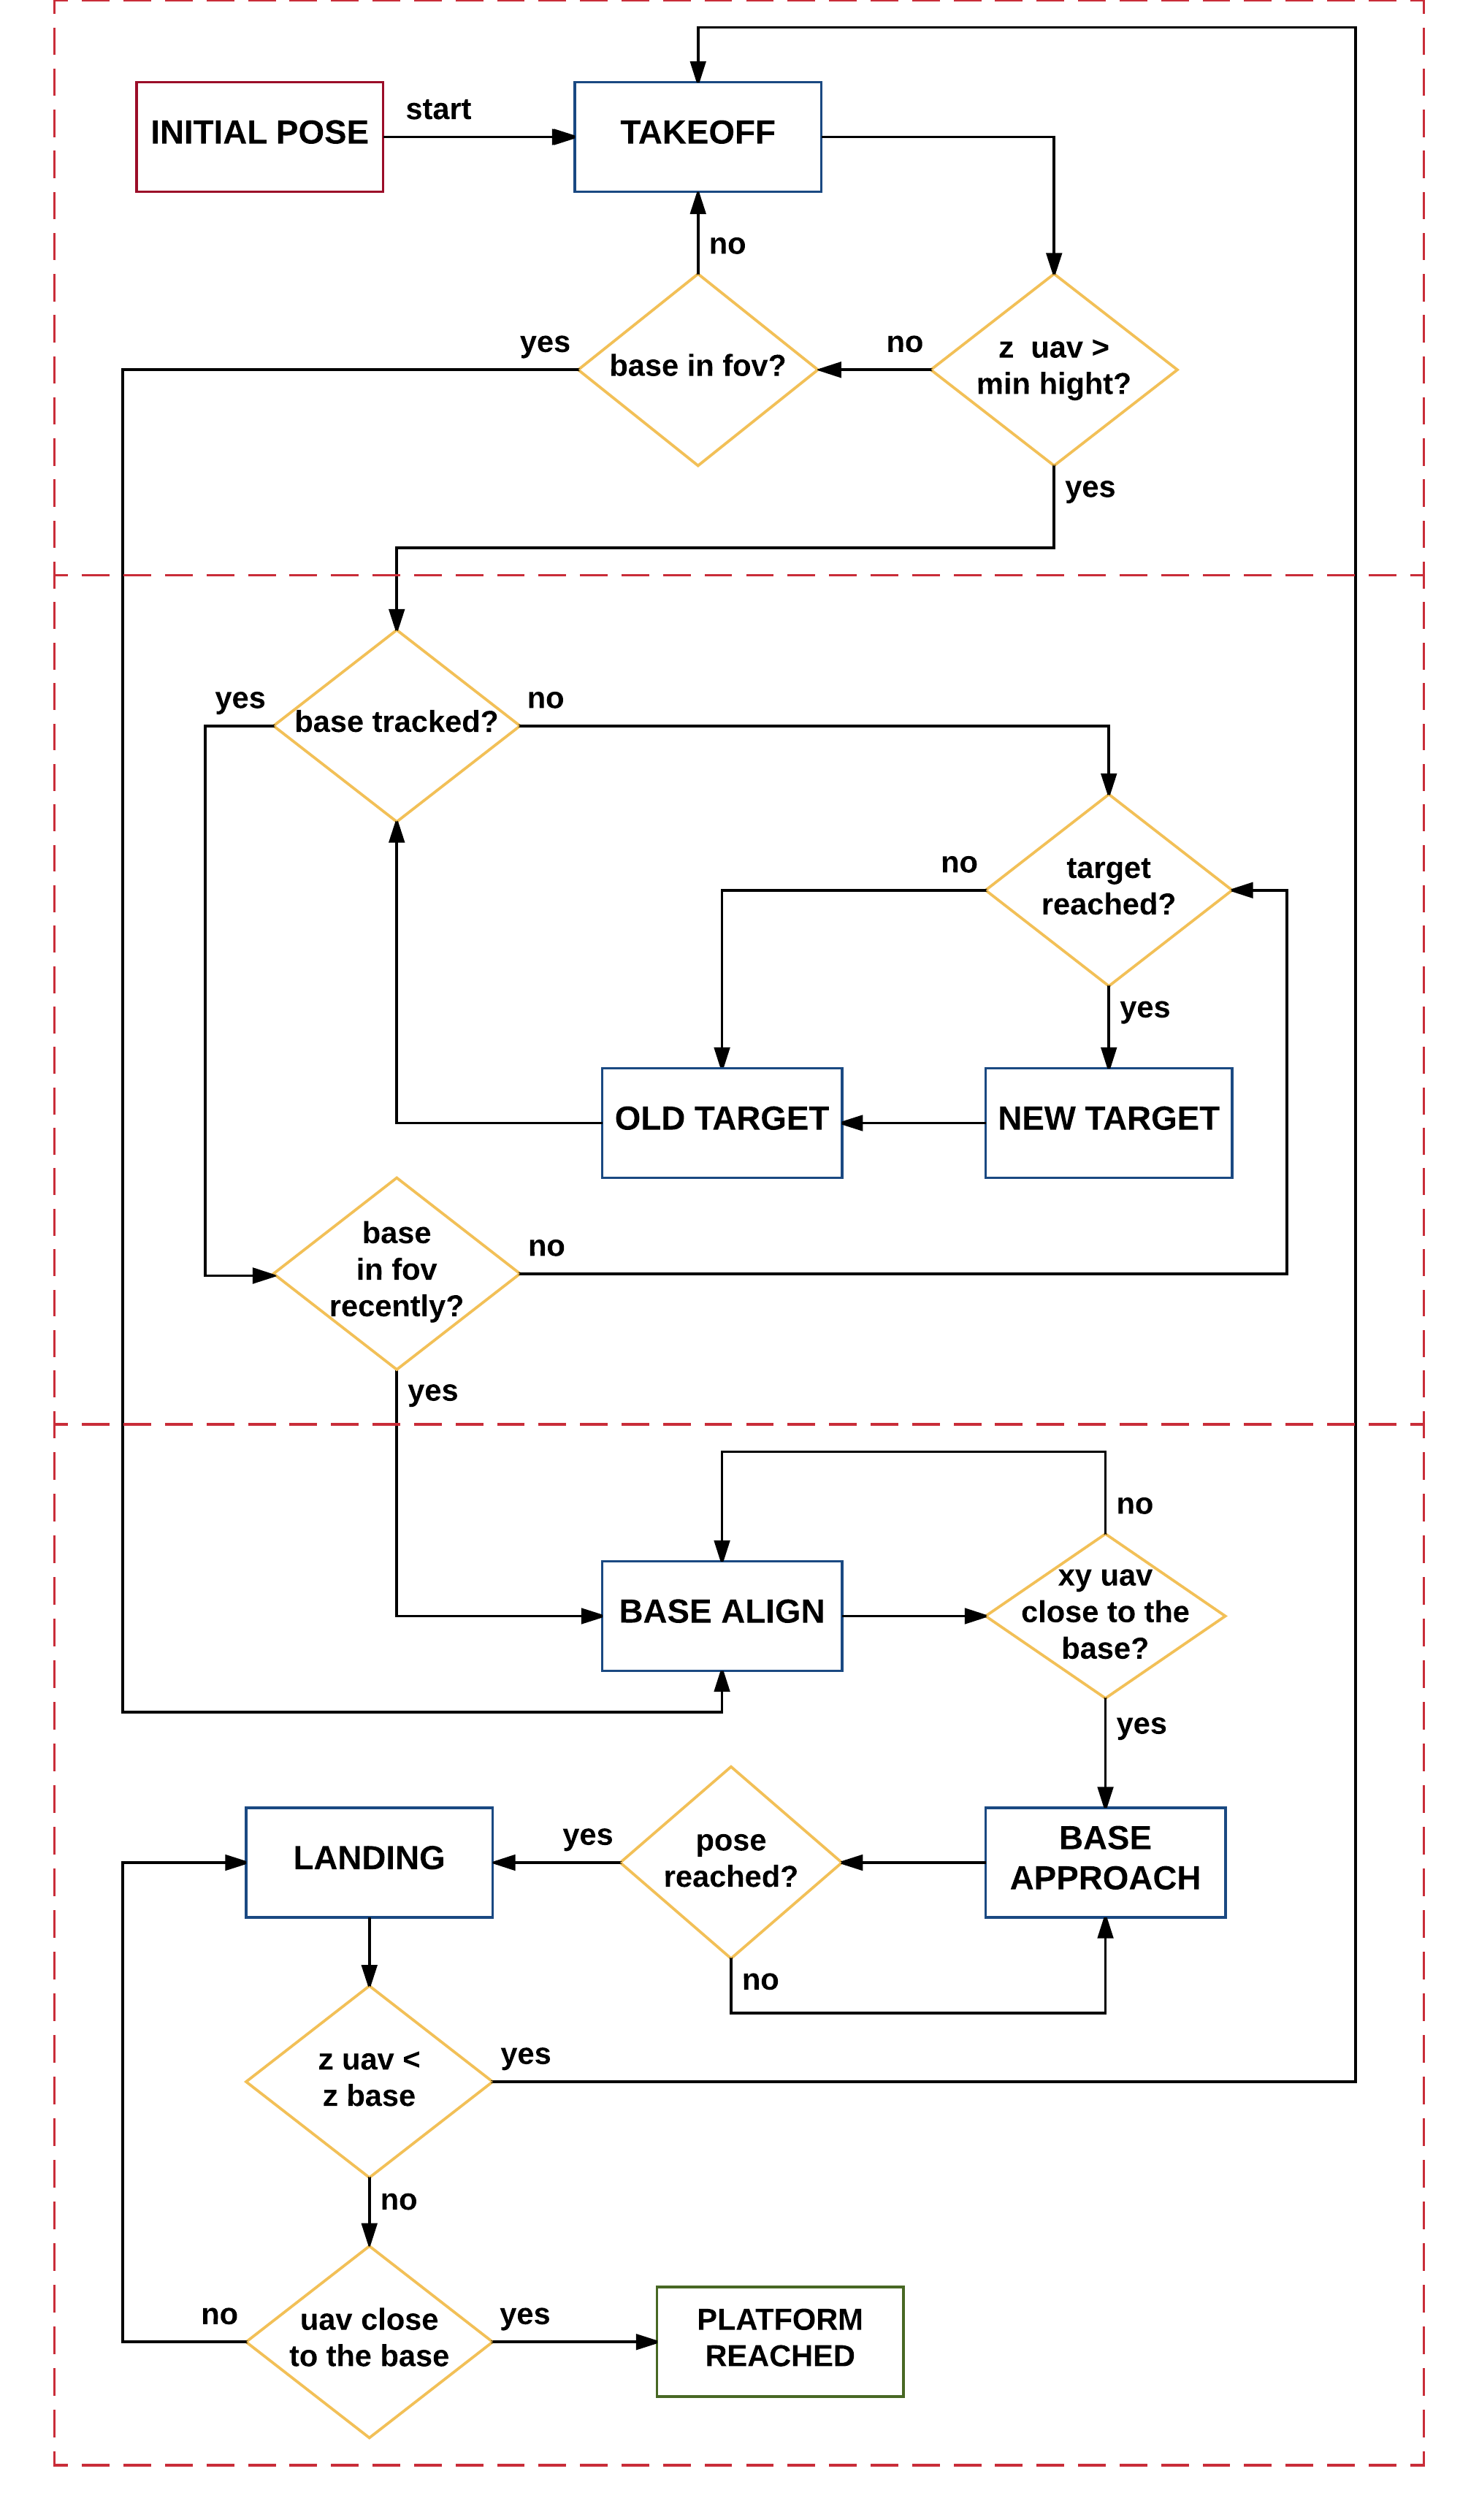
\includegraphics[width=0.97\textwidth]{img/area_exploration_state_machine.png}
    \caption{Area Exploration}
    \label{fig:area_exploration_state_machine}
\end{figure}

\subsection{Phases}
\subsubsection{First phase - Searching for the base}
In this phase the quadrotor starts from a given position and has to find the moving car.
Given the rectangle in which the platform can move the UAV follows a list of way-points in order to span the whole area at high altitude. In this way the downward camera can collect information from a large section of the space and the searching of the base is faster.\\
To find the platform we have the following assumptions:
\begin{itemize}
\item the platform is the only white square moving on the arena
\item in a small period of time the movement of the platform is approximable with a linear motion  
\end{itemize}

Base on these assumptions, we analyze the images from the down looking camera to find a moving white square and calculate its optical flow to predict its future position.
We perform the following passages:
\begin{itemize}
\item threshold the image in order to find the white features
\item find the edges with the canny edge algorithm
\item find the connected edges that define contours of shapes
\item select only the shapes with 4 edges
\item check if the edges have the same length 
\item check if the angle between edges is $\frac{\pi}{2}$
\end{itemize}
At this point we have the position of the squares in the image.\\
Now we try to calculate the optical flow of these points through the sequence of images and we track only the points that are moving with a velocity comparable to the one known. We can calculate the direction of the platform and then predict where it will be after a time $t$.
 

\subsubsection{Second phase - Approaching the base}

\subsubsection{Second phase - Following the base}

\subsubsection{Second phase - Landing on the base}
